\documentclass[titlepage,a4paper,12pt]{report}
\usepackage{amssymb,amsfonts,amsmath}
\usepackage{tikz}
\usetikzlibrary{arrows}
\newcommand\Interval[4]{%
  \begin{tikzpicture}[text height=1ex]%
    \draw[<-] (0,0) -- (1,0);
    \draw[{#3-#4}] (1,0) node[label=below:{#1}] {} -- (2,0) node[label=below:{#2}] {};
    \draw[->] (2,0) -- (3,0);
  \end{tikzpicture}
}
%\usepackage{fullpage}
\usepackage{graphicx}
%\usepackage[cc]{titlepic}
\usepackage{amsthm}
\newtheorem{definition}{Definition}[section]
\newtheorem{example}{Example}[section]
\newtheorem{theorem}{Theorem}[section]
\newtheorem{exercise}{Exercise}[section]
\newtheorem{corollary}{Corollary}[section]
\newtheorem{proposition}{Proposition}[section]
\pdfpagewidth 8.5in
\pdfpageheight 11in
\setlength\topmargin{-0.5in}
\setlength\headheight{0in}
\setlength\headsep{0in}
\setlength\textheight{9.5in}
\setlength\textwidth{7.0in}
\setlength\oddsidemargin{-0.5in}
\setlength\evensidemargin{1.0in}
\setlength\parindent{0.25in}
\setlength\parskip{0.25in}
%\begin{titlepage}
%\usepackage{titlepic}
%\titlepic{
\includegraphics[width=0.2\textwidth]{uz1.png}}
%
%\title{\textbf{HMTH111 Calculus 2}}
%\author{Nhawu. G\\
%		Department of Mathematics\\
%		University of Zimbabwe, ZIM}
%
%\end{titlepage}

\begin{document}
\begin{titlepage}
 
\begin{center}
 
 
% Upper part of the page

\includegraphics[width=0.15\textwidth]{uz1.png}\\[1cm]
 
\textsc{\LARGE University of Zimbabwe}\\[1.5cm]
 
\textsc{\Large HMTH101 CALCULUS 1}\\[0.5cm]
 
 
% Title

{ \huge \bfseries Calculus of Single Variables}\\[0.4cm]
 

 
% Author and supervisor
\begin{minipage}{0.4\textwidth}
\begin{center} \large
\emph{Author:}\\
G. \textsc{Nhawu}
\end{center}
\end{minipage}
\begin{minipage}{0.4\textwidth}
\begin{flushright} \large
\emph{Department:} \\
\textsc{Mathematics}
\end{flushright}
\end{minipage}

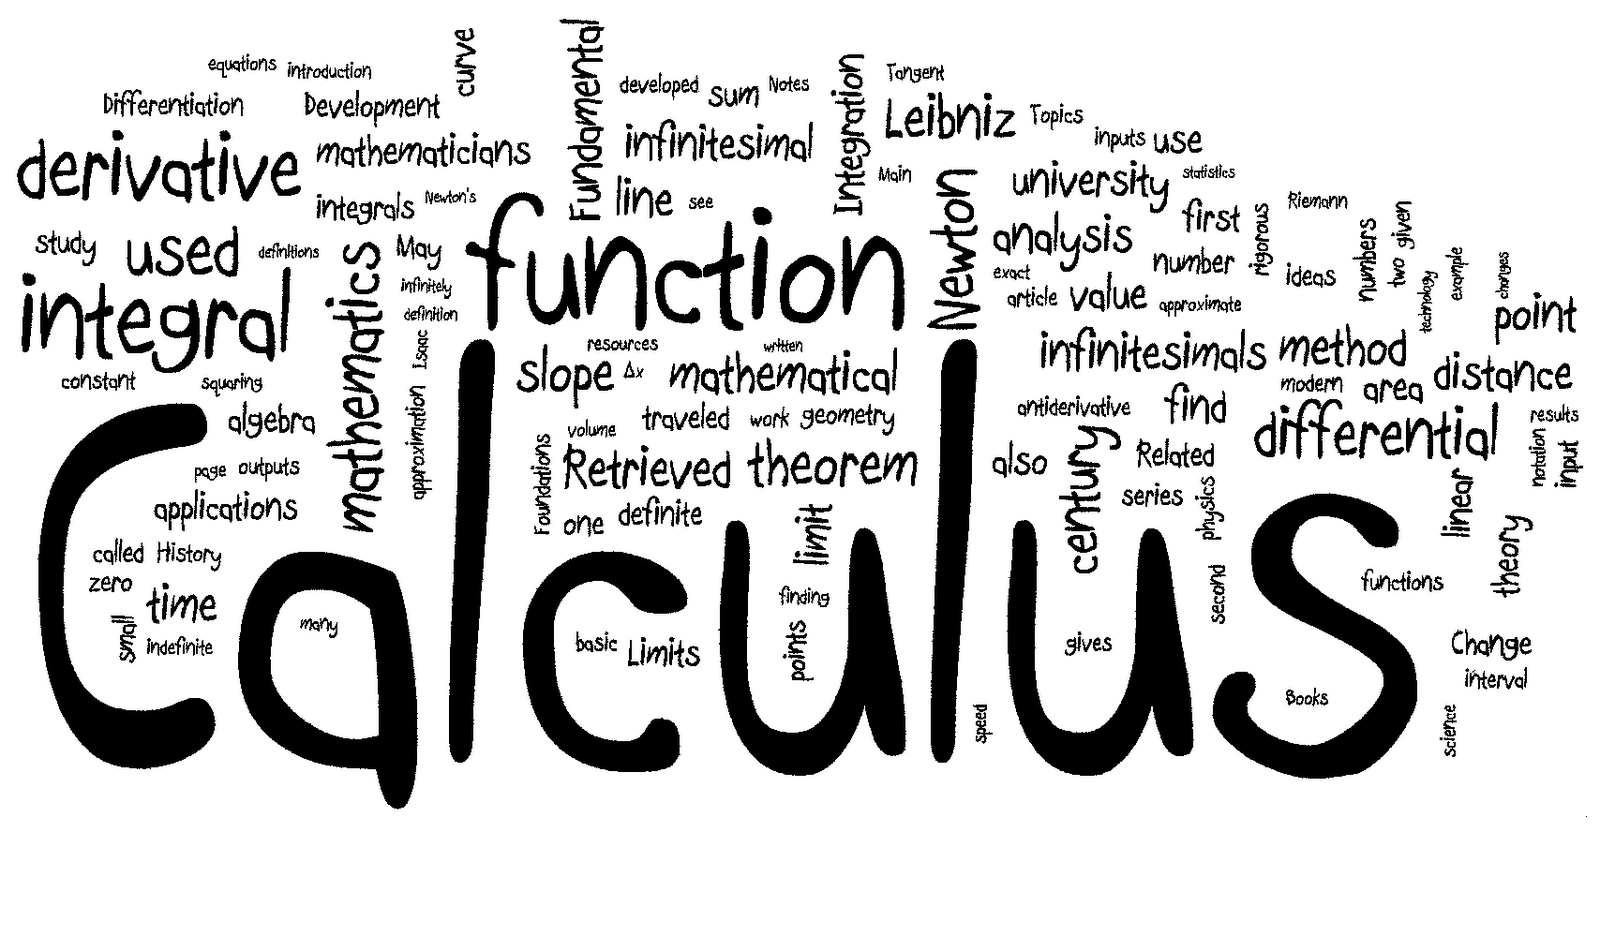
\includegraphics[width=0.98\textwidth]{calculus2.png}\\[1cm]
 \vfill
 
 
% Bottom of the page
{\large \today}
 
\end{center}
 
\end{titlepage}

\tableofcontents
\setcounter{chapter}{2}
\chapter{Sequences}
\begin{center}
	\small{\parbox{18cm}{
		\begin{raggedright}
		{\small
		\textit{A girl and a boy jump into a river. The boy swims over to the girl and says, ``God, it's cold." What's the probability they will kiss?}
 }
 
				\vspace{.5cm}\hfill{---Jenny Downham, You Against Me }
		\end{raggedright}
	}
} 
\end{center}
\begin{definition}
A \textbf{sequence} is a set of numbers $u_1, u_2, u_3, \dots$ in a definite order of arrangement and formed according to a definite rule.
\end{definition}
\noindent Each number in the sequence is called a \textit{term} and $u_n$ is called the \textit{$n$th term}. The sequence $u_1,u_2,u_3, \dots$ is written briefly as  $\{u_n\}$, e.g., $\{u_n\}=2n$, where $u_1=2$, $u_2=4$, $u_3=6$ and so on. A sequence can be \textit{finite} or \textit{infinite}. A finite sequence has only definite number of terms. An infinite sequence is non-terminating, e.g., $u_n=\dfrac{1}{2n-1}$.

\noindent \textbf{Recursive Definitions.} The values of the terms in a sequence may be given explicitly by formulas such as $u_n=n^3-73n$. 

\noindent A \textbf{recursive calculation} finds the value of $u_n$ by looking to see which terms $u_n$ depends on, then which terms depend, and so on.

\noindent \textbf{Example:} $u_0=1, \quad u_{n+1}=\dfrac{2}{u_n}, \quad n\in \mathbb{N}$.

\noindent \textbf{Solution:} 
\begin{eqnarray*}
u_1 &=& u_{0+1} = \dfrac{2}{u_0}=\dfrac{2}{1}=2\\
u_2 &=& u_{1+1}= \dfrac{2}{u_1} =\dfrac{2}{2}=1\\
u_3 &=& u_{2+1} = \dfrac{2}{u_2} =\dfrac{2}{1}=2.
\end{eqnarray*} 
\textbf{You Try It:} Define recursively 
\begin{equation*}
a_0=a_1=1, \quad \hbox{and} \quad a_n=a_{n-1}+2a_{n-2}, \, n\geq 2.
\end{equation*}
Find $a_6$ recursively.
\section{Limits of Sequences}
Lets consider the sequence $u_n=\dfrac{1}{n}$. The sequence has the terms $1, \frac{1}{2}, \frac{1}{3}, \frac{1}{4}, \dots$. We see that the terms of the sequence \textit{tend to} or \textit{approach} $0$.

\begin{definition}
A number $L$ is called the \textbf{limit} of an infinite sequence $a_1, a_2,a_3, \dots$ or $\{a_n\}$, if for any positive number $\varepsilon$, we can find a positive number $N$ depending on $\varepsilon$ such that $|a_n-L|<\varepsilon$ for all integers $n>N$. We write $\displaystyle \lim _{n\rightarrow \infty} a_n=L$.
\end{definition}
\noindent If $\{a_n\}$ is a convergent sequence, it means that the terms $a_n$ can be made arbitrarily close to $L$ for $n$ sufficiently large.
\begin{center}
 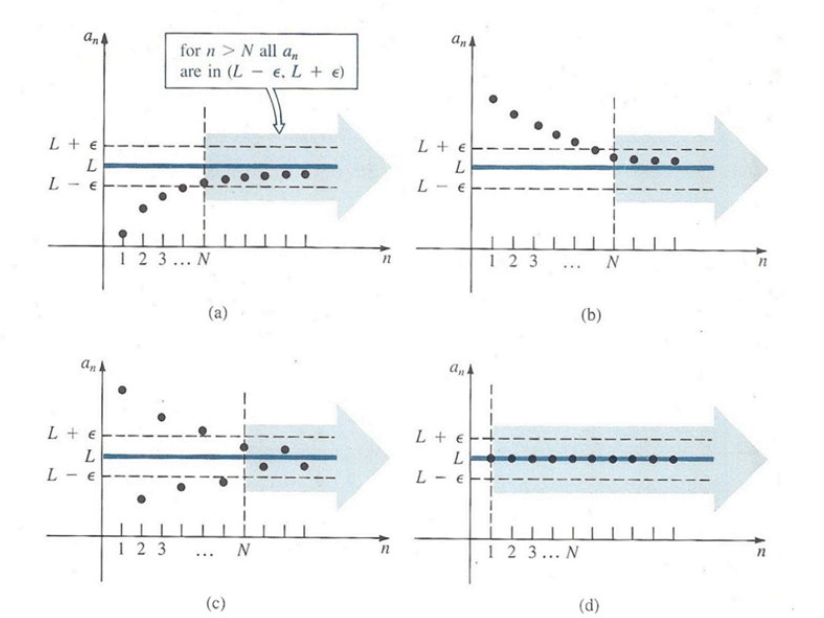
\includegraphics[width=0.7\textwidth]{seq.png}\\[1cm]
  \end{center}
\noindent \textbf{Example:} If $u_n=3+\dfrac{1}{n}=\dfrac{3n+1}{n}$, the sequence is $4, \frac{7}{2}, \frac{10}{3}, \dots$and we can show that \\ $\displaystyle \lim _{n\rightarrow \infty} u_n=3$.

\noindent If the limit of a sequence exists, the sequence is called \textbf{convergent}, otherwise, it is called \textbf{divergent}.

\noindent \textbf{Example:} Prove that $\displaystyle \lim _{n\rightarrow \infty} \frac{1}{n}=0$.

\noindent \textbf{Proof:} Let $\varepsilon >0$, we can find $N(\varepsilon)$ such that $\left|\dfrac{1}{n}-0\right|=\left|\dfrac{1}{n}\right|=\dfrac{1}{n} <\varepsilon$.  But $n>\dfrac{1}{\varepsilon}$. So $N=\dfrac{1}{\varepsilon}$. Taking $N$ to be the smallest integer greater than $ \dfrac{1}{\varepsilon}$, we have, $\displaystyle \lim _{n\rightarrow \infty} \dfrac{1}{n}=0$.

\noindent \textbf{You Try It:} Prove that $\displaystyle \lim _{n\rightarrow 0} \dfrac{1}{n^p}=0$ if $p\in \mathbb{N}$.

\noindent \textbf{Example:} Use the definition of a limit to prove that $\displaystyle \lim _{n\rightarrow \infty} \dfrac{2n-1}{3n+2}=\dfrac{2}{3}$.

\noindent \textbf{Proof:} Let $\varepsilon >0$, we can find $N(\varepsilon)$ such that 
\begin{equation*}
\left|\dfrac{2n-1}{3n+2}-\dfrac{2}{3}\right| =\left|\dfrac{3(2n-1)-2(3n+3)}{3(3n+2)}\right| =\left|\dfrac{6n-3-6n-4}{3(3n+2)}\right|=\left|\dfrac{-7}{3(3n+2)}\right|= \left|\dfrac{7}{3(3n+2)}\right|<\varepsilon 
\end{equation*}
\begin{eqnarray*}
\dfrac{7}{3(3n+2)} &<& \varepsilon \\
n &>& \dfrac{7-6\varepsilon}{9\varepsilon}.
\end{eqnarray*}
Take $N=\dfrac{7-6\varepsilon}{9\varepsilon}$. So taking $N$ to be the smallest integer greater than $\dfrac{7-6\varepsilon}{9\varepsilon}$, we have \\ $\left|\dfrac{2n-1}{3n+2}-\dfrac{2}{3}\right|<\varepsilon$ , i.e., $\displaystyle \lim _{n\rightarrow \infty} \dfrac{2n-1}{3n+2}=\dfrac{2}{3}$.
\section{Theorems on Limits}
If $\displaystyle \lim _{n\rightarrow \infty} a_n =A$ and $\displaystyle \lim _{n\rightarrow \infty} b_n =B$, then 
\begin{enumerate}
\item $\displaystyle \lim _{n\rightarrow \infty} (a_n +b_n) = \lim _{n\rightarrow \infty} a_n + \lim _{n\rightarrow \infty} b_n =A +B$.
\item $\displaystyle \lim _{n\rightarrow \infty} (a_n-b_n) = \lim _{n\rightarrow \infty} a_n-\displaystyle \lim _{n\rightarrow \infty} b_n =A-B$.
\item $\displaystyle \lim _{n\rightarrow \infty} (a_n\cdot b_n)=(\lim _{n\rightarrow \infty} a_n)(\lim _{n\rightarrow \infty} b_n)=AB$.
\item $\displaystyle \lim _{n\rightarrow \infty} \dfrac{a_n}{b_n}=\dfrac{\displaystyle \lim _{n\rightarrow \infty} a_n}{\displaystyle \lim _{n\rightarrow \infty} b_n} =\dfrac{A}{B}$ if $\displaystyle \lim _{n\rightarrow \infty} b_n =B\neq 0$.
\item The limit of a convergent sequence $\{u_n\}$ of real numbers is unique. 
\end{enumerate}
\noindent \textbf{Proof:} We must show that if $\displaystyle \lim _{n\rightarrow \infty} u_n=l_1$ and $\displaystyle \lim _{n\rightarrow \infty} u_n=l_2$, then $l_1=l_2$. By \textit{hypothesis}, given any $\varepsilon >0$, we can find $N$ such that $|u_n-l_1|<\dfrac{\varepsilon}{2}$ when $n>N$ and $|u_n-l_2|<\dfrac{\varepsilon}{2}$ when $n>N$. Then 
\begin{equation*}
|l_1-l_2|=|l_1-u_n+u_n-l_2| \leq |l_1-u_n|+|u_n-l_2|<\dfrac{\varepsilon}{2}+\dfrac{\varepsilon}{2}=\varepsilon , 
\end{equation*}
i.e., $|l_1-l_2|$ is less than any positive $\varepsilon$ (however small) and so must be zero, i.e., $l_1-l_2=0\Longrightarrow l_1=l_2$.

\noindent \textbf{Example:} If $\displaystyle \lim _{n\rightarrow \infty} a_n=A$ and $\displaystyle \lim _{n\rightarrow \infty} b_n=B$, prove that $\displaystyle \lim _{n\rightarrow \infty} (a_n +b_n )=A+B$.

\noindent \textbf{Proof:} We must show that for any $\varepsilon >0$, we can find $N>0$, such that $|(a_n+b_n)-(A+B)|<\varepsilon$ for all $n>N$. We have 
\begin{equation*}
|(a_n+b_n)-(A+B)|=|(a_n-A)+(b_n-B)| \leq |a_n-A| +|b_n-B|.
\end{equation*} 
By \textit{hypothesis}, given $\varepsilon >0$ we can find $N_1$ and $N_2$ such that $|a_n-A|<\dfrac{\varepsilon}{2}$ for all $n>N_1$ and $|b_n-B|<\dfrac{\varepsilon}{2}$ for all $n>N_2$. Then 
\begin{equation*}
|(a_n+b_n)-(A+B)|<\dfrac{\varepsilon}{2} +\dfrac{\varepsilon}{2}=\varepsilon
\end{equation*}
for all $n>N$ where $N=\max (N_1, N_2)$. Hence $\displaystyle \lim _{n\rightarrow \infty}(a_n+b_n)=A+B$.
\section{Sequences Tending to Infinity}
$n$ tends to infinity, $n\rightarrow \infty $ ($n$ grows or increases beyond any limit ). Infinity is not a number and the sequences that tend to infinity are not convergent.

\noindent We write $\displaystyle \lim _{n\rightarrow \infty} a_n=\infty$, if for each positive number $M$, we can find a positive number $N$ (depending on $M$) such that $a_n>M$ for all $n>N$.

\noindent Similarly, we write $\displaystyle \lim _{n\rightarrow \infty} a_n=-\infty$, if for each positive number $M$, we can find a positive number $N$ such that $a_n<-M$ for all $n>N$.

\noindent \textbf{Example:} Prove that (a)\, $\displaystyle \lim _{n\rightarrow \infty} 3^{2n-1}=\infty$ \quad (b)\, $\displaystyle \lim _{n\rightarrow \infty} (1-2n)=-\infty$.

\noindent \textbf{Proof:} (a)\, If for each positive number $M$ we can find a positive number $N$ such that $a_n>M$ for all $n>N$, then $3^{2n-1}>M$ when $(2n-1)\ln 3 >\ln M$, i.e., $n>\dfrac{1}{2}\left(\dfrac{\ln M}{\ln 3}+1\right)$. Taking $N$ to be the smallest greater than $\dfrac{1}{2}\left(\dfrac{\ln M}{\ln 3}+1\right)$, then $\displaystyle \lim _{n\rightarrow \infty} 3^{2n-1}=\infty$.

\noindent (b)\, If for each positive number $M$, we can find a positive number $N$ such that $a_n<-M$ for all $n>N$, i.e., $1-2n<-M$ when $2n-1>M$ or $n>\frac{1}{2}(M+1)$. Taking $N$ to be the smallest integer greater than $\frac{1}{2}(M+1)$, we have $\displaystyle \lim _{n\rightarrow \infty} (1-2n)=-\infty$.

\section{Bounded and Monotonic Sequences}
A sequence that tends to a limit $l$ is said to be convergent and the sequence converges to $l$. A sequence may tend to $+\infty $ or $-\infty$, and is said to be divergent and it diverges to $+\infty $ or $-\infty$.

\noindent If $u_n\leq M$ for $n=1,2,3, \dots$, where $M$ is a constant, we say that the sequence $\{u_n\}$ is \textit{bounded above} and $M$ is called an \textit{upper bound}. The smallest upper bound is called the \textit{least upper bound} (l.u.b).

\noindent If $u_n\geq m$, the sequence is \textit{bounded below} and $m$ is called a \textit{lower bound}. The largest lower bound is called the \textit{greatest lower bound} (g.l.b).

\noindent If $m\leq u_n\leq M$, the sequence is called \textit{bounded}, indicated by $|u_n|\leq P$. (Every convergent sequence is bounded, but the converse is not necessarily true)

\noindent If $u_{n+1}\geq u_n$, the sequence is called \textit{monotonic increasing} and if $u_{n+1}>u_n$ it is called \textit{strictly increasing}. If $u_{n+1}\leq u_n$, the sequence is called \textit{monotonic decreasing}, while if $u_{n+1}<u_n$ it is \textit{strictly decreasing}.

\noindent \textbf{Examples:} $1.$\, The sequence $1, 1.1, 1.11, 1.111, \dots$ is bounded and monotonic increasing.\\
$2.$ The sequence $1,-1,1,-1,1,\dots$ is bounded but not monotonic increasing or decreasing.
\begin{definition}
A \textbf{null sequence} is a sequence that converges to $0$, e.g., $u_n=\dfrac{1}{n-10}, \, n\geq 11$.
\end{definition}
\noindent If $\{u_n\}$ does not tend to a limit or $+\infty$ or $-\infty $, we say that $\{u_n\}$ \textit{oscillates} (or is an oscillating sequence). It can oscillate finitely (bounded) or infinitely (unbounded).

\noindent \textbf{Examples:} $u_n=(-1)^n$, \quad $u_n=(-1)^n n$.

\section{Limits of Combination of Sequences}
We want to be able to evaluate limits, for example, of the form $\displaystyle \lim _{n\rightarrow \infty}\left(2-\frac{1}{n}+\frac{3}{n^2}\right)$ or $\displaystyle \lim _{n\rightarrow \infty} \dfrac{5-2n^2}{4+3n+2n^2}$.

\noindent \textbf{Example:} $\displaystyle \lim _{n\rightarrow \infty}\left(2-\frac{1}{n}+\frac{3}{n^2}\right)=\lim _{n\rightarrow \infty} 2-\lim _{n\rightarrow \infty}\frac{1}{n}+3\lim _{n\rightarrow \infty}\frac{1}{n^2}=2-0+0=2$.

\noindent \textbf{Example:} $\displaystyle \lim _{n\rightarrow \infty} \dfrac{3n^2-5n}{5n^2+2n-6}=\lim _{n\rightarrow \infty} \dfrac{3-\frac{5}{n}}{5+\frac{2}{n}-\frac{6}{n^2}}=\dfrac{3+0}{5+0+0}=\dfrac{3}{5}$.

\noindent \textbf{Example:} $\displaystyle \lim _{n\rightarrow \infty}(\sqrt{n+1}-\sqrt{n})=\lim _{n\rightarrow \infty}(\sqrt{n+1}-\sqrt{n})\cdot \left(\dfrac{\sqrt{n+1}+\sqrt{n}}{\sqrt{n+1}+\sqrt{n}}\right)=\lim _{n \rightarrow \infty}\dfrac{1}{\sqrt{n+1}+\sqrt{n}}=0$.
\section{Squeeze Theorem}
If $\displaystyle \lim _{n\rightarrow \infty} a_n=l=\lim _{n\rightarrow \infty}b_n$ and there exists an $N$ such that $a_n\leq c_n\leq b_n$, for all $n>N$, then $\displaystyle \lim _{n\rightarrow \infty}c_n=l$.

\noindent \textbf{Example:} Find $\displaystyle \lim _{n\rightarrow \infty} \dfrac{\cos n}{n}$.

\noindent \textbf{Solution:} We know that $-1\leq \cos n\leq 1\\
 \Longrightarrow -\dfrac{1}{n}\leq \dfrac{\cos n}{n}\leq \dfrac{1}{n}\Longrightarrow \displaystyle -\lim _{n\rightarrow \infty}\dfrac{1}{n}\leq \lim _{n\rightarrow \infty}\dfrac{\cos n}{n}\leq \lim _{n\rightarrow \infty}\dfrac{1}{n}\Longrightarrow 0\leq \displaystyle \lim _{n\rightarrow \infty}\dfrac{\cos n}{n} \leq 0\\
 \Longrightarrow \displaystyle \lim _{n\rightarrow \infty} \dfrac{\cos n}{n}=0$.
 \section{Tutorial Questions}
 \begin{enumerate}
\item Write the first five terms of each of the following sequences.\\
(i)\, $\Biggl \{\dfrac{2n-1}{3n+2}\Biggr \}$ \quad (ii)\, $\Biggl\{\dfrac{1-(-1)^n}{n^3}\Biggr\}$ \quad (iii)\,$\Biggl \{\dfrac{(-1)^{n-1}}{2\cdot 4 \cdot 6 \cdots 2n}\Biggr\}$  \quad (iv)\, $\Biggl \{\dfrac{(-1)^{n-1}x^{2n-1}}{(2n-1)!}\Biggr \}$ \\ (v)\, $\Biggl \{\dfrac{1}{2} +\dfrac{1}{4}+\dfrac{1}{8}+\cdots +\dfrac{1}{2^n}\Biggr\}$ \quad (vi)\, $\Biggl \{\dfrac{\cos nx}{x^2+n^2}\Biggr \}$ \quad (vii)\, $\Biggl \{\dfrac{\sqrt{n}}{n+1}\Biggr \}$.
\item Determine the general term of each sequence.
\begin{itemize}
\item[(i)] $\dfrac{1}{2}, \dfrac{2}{3}, \dfrac{3}{4}, \dfrac{4}{5}, \dfrac{5}{6}, \dots$. 
\item[(ii)] $\dfrac{1}{2}, \dfrac{1}{12}, \dfrac{1}{30}, \dfrac{1}{56}, \dfrac{1}{90}, \dots$.
\item[(iii)] $\dfrac{1}{5^3}, \dfrac{3}{5^5}, \dfrac{5}{5^7}, \dfrac{9}{5^{11}}, \dots$.
\end{itemize}
\item \begin{itemize}
\item[(i)] Recursively define $b_0=b_1=1$ and $b_n=2b_{n-1}+b_{n-2}, n\geq 2$. Calculate $b_5$.
\item[(ii)] Recursively define $a_0=0, a_1=1, a_2=2$ and $a_n=a_{n-1}-a_{n-2}+a_{n-3}$ for $n\geq 3$. List the first five terms.
\item[(iii)] Recursively define $s_0=1, s_1=-3$ and $s_n=6s_{n-1}-9s_{n-2}$ for $n \geq 2$, find $s_5$.
\end{itemize}
\item Find the least positive integer $N$ such that $\left|\dfrac{(3n+2)}{(n-1)}-3\right|<\varepsilon$ for all $n>N$ if \\
(i)\, $\varepsilon =0.01$ \quad (ii)\, $\varepsilon =0.001$ \quad (iii)\, $\varepsilon = 0.0001$.
\item Use the definition of limits to show that $\displaystyle \lim _{n\rightarrow \infty}\dfrac{2n-1}{3n+4}$ \textbf{cannot} be $\dfrac{1}{2}$.
\item If $\displaystyle \lim _{n\rightarrow \infty} a_n =A$ and $\displaystyle \lim _{n\rightarrow \infty} b_n=B$, prove that  $\displaystyle \lim _{n\rightarrow \infty}(a_n \cdot b_n)=AB$ and  $\displaystyle \lim _{n\rightarrow \infty}\dfrac{a_n}{b_n}=\dfrac{A}{B}$ if $\displaystyle \lim _{n\rightarrow \infty} b_n =B \neq 0$.
\item Use the definition of a limit to verify each of the following limits.\\
(i)\, $\displaystyle \lim _{n\rightarrow \infty}\dfrac{2n-1}{3n+2}=\dfrac{2}{3}$ \quad  (ii)\, $\displaystyle \lim _{n\rightarrow \infty}\dfrac{4-2n}{3n+2}=-\dfrac{2}{3}$ \quad (iii)\, $\displaystyle \lim _{n\rightarrow \infty}\dfrac{\sin n}{n}=0$ \\
 (iv)\, $\displaystyle \lim _{n\rightarrow \infty}(5n-2)=\infty$ \quad (v)\, $\displaystyle \lim _{n\rightarrow \infty}\dfrac{c}{n^p}=0,\, \mbox{where}~~ c\neq 0, p>0$ \\ (vi)\, $\displaystyle \lim _{n\rightarrow \infty}(1-2n)=-\infty$ \quad (vii)\,  $\displaystyle \lim _{n\rightarrow \infty} a^n=0$ where $0< |a|<1$. 
 \item Use the properties of limits to evaluate each of the following limits.\\
 (i)\, $\displaystyle \lim _{n\rightarrow \infty}\dfrac{4-2n-3n^2}{2n^2+n}$ \quad (ii)\, $\displaystyle \lim _{n\rightarrow \infty}\left( \dfrac{\sqrt{3n^2-5n+4}}{2n-7}\right )$ \quad (iii)\, $\displaystyle \lim _{n\rightarrow \infty}(\sqrt{n^2+n}-n )$\\ (iv)\, $\displaystyle \lim _{n\rightarrow \infty}\left(\dfrac{n(n+2)}{n+1}-\dfrac{n^3}{n^2+1} \right)$ \quad (v)\, $\displaystyle \lim _{n\rightarrow \infty}(\sqrt{n+1}-n)$ \quad (vi)\, $\displaystyle \lim _{n\rightarrow \infty}\left(\dfrac{2n-3}{3n+7}\right)^4$ \\ (vii)\, $\displaystyle \lim _{n\rightarrow \infty}(\sqrt{4n^2+n+5}-2n)$ \quad (viii)\, $\displaystyle \lim _{n\rightarrow \infty}\sqrt[3]{\dfrac{(3-\sqrt{n})(\sqrt{n}+2)}{8n-4}}$.
 \item If $u_{n+1}=\frac{1}{2}(u_n+\frac{2}{u_n})$ where $u_1>0$, show that $\displaystyle \lim _{n\rightarrow \infty}u_n=\sqrt{2}$.
 \item \begin{itemize}
 \item[(i)] If a sequence $\{u_n\}$ is recursively defined by $u_{n+1}=\sqrt{u_n+1}, u_1=1$, prove that\\ $\displaystyle \lim _{n\rightarrow \infty}u_n=\frac{1}{2}(1+\sqrt{5})$.
 \item[(ii)] Show by induction that the sequence $\{u_n\}$ is bounded above by $2$.
 \item[(iii)] Show by induction that $\{u_n\}$ is monotonic increasing.
 \end{itemize}
 \item 
 \begin{itemize}
 \item[(i)] Let $\{x_n\}$ be the sequence defined by $x_1=1, x_{n+1}=\sqrt{3x_n+1}$ for all $n\geq 1$. Prove that $\{x_n\}$ is an increasing function for every $n$.
 \item[(ii)] Show that the sequence has $\dfrac{7}{2}$ as an upper bound i.e. $x_n \leq \dfrac{7}{2}$ for all $n$.
 \end{itemize}
 \item Show that if $a_n\rightarrow l$ as $n\rightarrow \infty$, then $a_{n+1}=\dfrac{2}{3}a_n +\dfrac{2}{3a_n ^2}$ converges to $\sqrt[3]{2}$.
 \item Let $a_n=\sqrt{n+1}-\sqrt{n}$. Show that $a_n\rightarrow 0$ as $n\rightarrow \infty$.
 \item A sequence $\{u_n\}$ is such that $u_{n+3}=6u_{n+2}-5u_{n+1}$ and $u_1=2, u_2=6$. Prove that\\ $u_n=5^{n-1}+1$.
 \item A sequence $\{a_n\}$ is such that $a_1=1, a_2=3$ and $a_{n+2}=3a_{n+1}-2a_n$. Prove that $a_n=2^n-1$.
 \item Define a sequence $x_1, x_2, x_3, \dots$ by $x_1=5, x_2=13$ and $x_{n+1}=5x_n-6x_{n-1}$. Prove by induction that $x_n=2^n+3^n$.
 \item Define a sequence $\{x_n\}$ recursively by $x_1=1$ and $x_{n+1}=\sqrt{2+x_n}$.
 \begin{itemize}
 \item[(i)] Show that $\{x_n\}$ is a monotone increasing sequence.
 \item[(ii)] Show that the sequence is bounded above by $2$.
 \item[(iii)] State why the sequence converges.
 \item[(iv)] Find the limit of the sequence.
 \end{itemize}
\end{enumerate}
\end{document}